The data yields and backgrounds estimation for all 84 search bins are showed in the Fig~\ref{fig:84sbunblind}. No statistically significant excess is observed. \ttbar, $W$+jets and single top are the largest source of the background. The $Z$+jets can be dominant in the high met search bins. The QCD and rare processes are small for all search bins. 

\begin{figure}[htbp]
 \begin{center}
  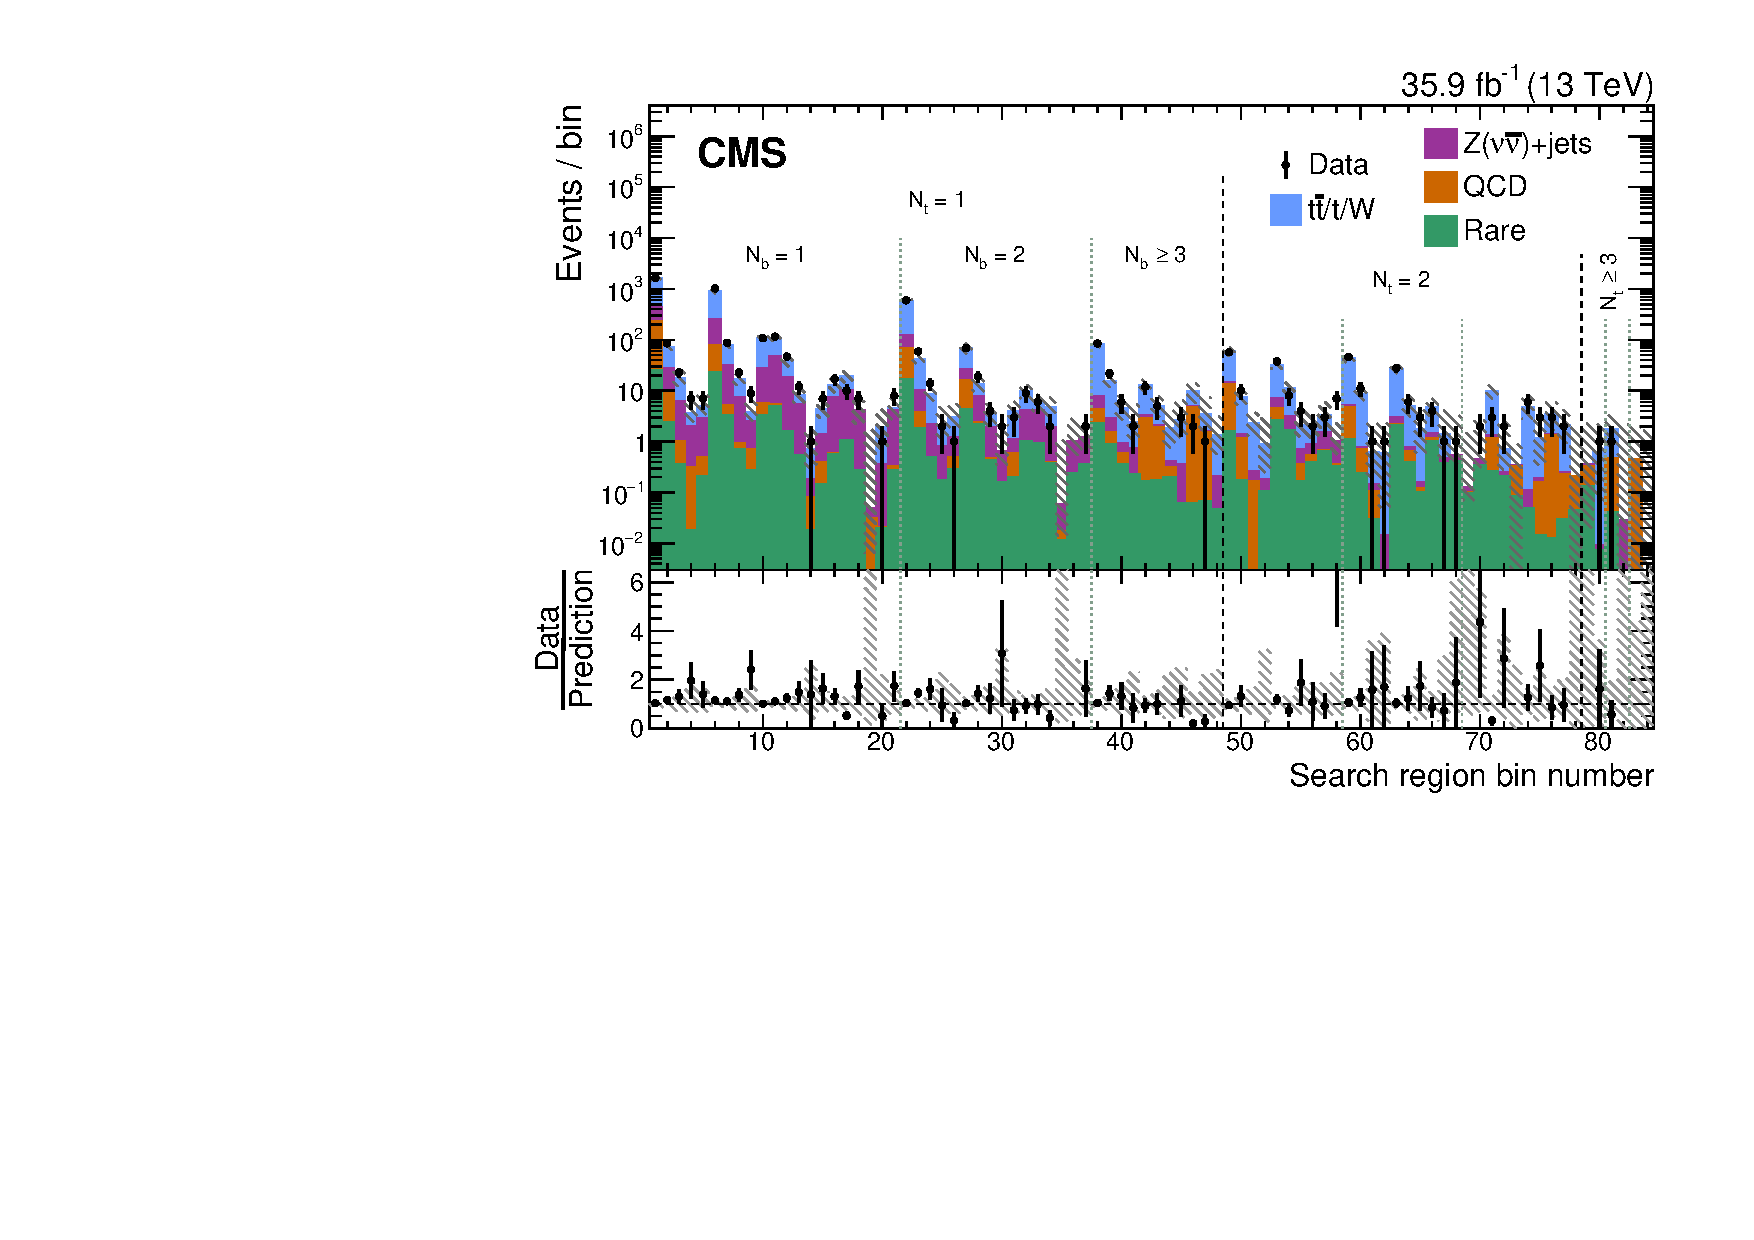
\includegraphics[width=0.8\textwidth]{sections/mc4/Results/figures/UnblindPlots.pdf}
 \end{center}
 \caption{Observed event yields in data (black points) and predicted SM background (filled solid area) for the 84 search bins. The lower panel shows the ratio of data over total background prediction in each search bin. For both panels, the error bars show the statistical uncertainty associated with the observed data counts, and the grey (blue) hatched bands indicate the statistical (systematic) uncertainties in the total predicted background.}
 \label{fig:84sbunblind}
\end{figure}

The analysis is interpreted as the upper limit of the signal model cross section. The upper limit of the signal model cross sections with 95\% confidence level are calculated, using modified frequentist ($CL_{s}$) approach\cite{Cowan:2010js}. The $CL_{s}$ is defined in the Eq~\ref{eq:c4cls}:

\begin{equation}
 \begin{aligned}
  CL_{s}=\frac{CL_{s+b}}{CL_{b}}
 \end{aligned}
 \label{eq:c4cls}
\end{equation}

Where the $CL_{s+b}$ is the confidence level in signal plus background hypothesis, and $CL_{b}$ is confidence level with the background only assumption. 

In the $CL_{s+b}$ calculation, we assume that the observed number of events n to follow Poisson distribution with an expected value $E[n]=\mu s+b$. The s is the mean number of events from a signal model, which is a known number from simulation. The b is the expected number of background, also a known number. The $\mu$ is the signal acceptance, which is the value we need to obtain with likelihood. 

The b is the expected numbers from all backgrounds. We treat them as a nuisance parameter, whose value is constraint by the control samples (e.g. single muon control sample for lost lepton and hadronic tau, inverted $\Delta \phi$ for QCD, etc.). The control samples are also a Poisson distribution with mean value $E[n]=\tau b$. The $\tau$ is the scale factors between the control sample region and signal region, for example, the translation factors in QCD case. Therefore the likelihood function for mu and b can be expressed in Eq~\ref{eq:c4clslikelihood}:

\begin{equation}
 \begin{aligned}
  L(\mu,b)= \frac{(\mu s+b)^{n}}{n!}e^{-(\mu s+b)} \prod_{k=1}^{M}\frac{b_{k}^{m_{k}}}{m_{k}!}e^{-b_{k}}
 \end{aligned}
 \label{eq:c4clslikelihood}
\end{equation}

The M is the total number of backgrounds. In this analysis, M=4: one for lost lepton and hadronic tau, the rest three are $Z$+jets, QCD and Rare. The likelihood is maximized following the procedure described in\cite{Cowan:2010js}.

We consider the following uncertainties in the signal cards: 

\begin{itemize}
\item {\bf MC statistics:} statistical uncertainties from MC signal samples.
\item {\bf Luminosity:} a 2.6\% flat contribution is assigned.
\item {\bf lepton veto:} lepton vetos are categorized as POG muon and electron veto, muon and electron track veto and pion track veto.
The number of signal events vetoed by each of the categories are evaluated. Then the yields are varied by the corresponding veto category uncertainties and propogated to be relative changes to the signal yields in the search bins as lepton veto uncertainties. Here the amount of veto'ed events effectively reflects the various lepton selection efficiency.
The efficiency uncertainties on the lepton selections either come from the lepton SF group (for muon and electron efficiency) or dedicated studies by either the lost lepton (for muon and electron track efficiency) or the hadronic tau method (for pion track efficiency). The Moriond results from the lepton SF group are used.
\item {\bf b-tag efficiency:} the b-tagging and mistagging scale factors are functions of the jet $p_{T}$ and $\eta$.
\item {\bf b-tag FastSim corrections:} The b-tagging and mistagging performance as derived from fast simulation is corrected to match the
full simulation predictions. Separate correction factors are derived for b-jets, c-jets, and light-flavor-jets, as a function of the jet $p_{T}$ and $\eta$. As with the scale factors above, the correction factors for each type of jet are varied independently within their uncertainties and propagated to the signal bins.  Currently, the correction factors and uncertainties are derived from an average mixture of \ttbar and signal events.
\item {\bf Trigger efficiency:} The signal samples are corrected for the trigger inefficiencies. And the effect of trigger efficiency uncertainties on the signal samples is at most a 2.6\% in the lowest \MET bins.
\item {\bf Pileup acceptance:}
The signal acceptance was found not to depend strongly on pileup, and an uncertainty is assigned to quantify this. The relative signal acceptance as a function of $n_{\text{vtx}}$ is modeled from Monte Carlo, and is applied to the normalized $n_{\text{vtx}}$ distribution from observed data.
The relative signal acceptance is modeled as a linear fit in two bins, $n_{\text{vtx}} < 20$ (low PU) or $n_{\text{vtx}} \geq 20$ (high PU). A confidence band for the linear fit is derived from the uncertainty on the relative acceptance due to statistical uncertainty on the Monte Carlo event counts. The pileup acceptance uncertainty is found by calculating the expectation
value:
\begin{equation}
c = \sum_{n_{\text{vtx}}=0}^{100} f_{\text{MC}}(n_{\text{vtx}})g_{\text{data}}(n_{\text{vtx}}) \label{eq:puacc-expval}
\end{equation}
where $f_{\text{MC}}$ is taken from the central fit value or the lower or upper limit from the confidence band.
$g_{\text{data}}(n_{\text{vtx}})$ is measured in a single electron control region (requiring $\njets\geq2$, $n_{\text{electron}}=1$, and \texttt{HLT\_Elea27\_WPTight}).
The up and down variations of c are normalized to the value from the central variation of the fit. The magnitude of the uncertainty is found to be 0.2-4.1\%
\item {\bf Renormalization and factorization scales:} the uncertainty is calculated using the envelope of the weights obtained from varying the renormalization and factorization scales, $\mu_{R}$ and $\mu_{F}$, by factor of two \cite{Cacciari:2003fi,Catani:2003zt}. The scales' effects on signal shapes are considered as their uncertainties on signal cross-sections are taken care of separately. %The effect on the T2tt signal samples ranges from 0 to 2.9\%.
\item {\bf ISR:} The ISR correction is applied and its uncertainty is propagated following the procedure of recommendation for Moriond 2017.
\item {\bf Jet Energy Corrections:} The jet energy corrections (JEC) are varied within the $p_{T}$ and $\eta$-dependent jet energy scale uncertainties available in the official database. A different set of corrections and uncertainties are used in fast simulation samples.  These variations are propagated into the jet-dependent search variables, such as: \nbjets, \ntops, \MET, \MTTwo, \HT, $\Delta\phi(\MET,j_{i})$.
\item {\bf \MET uncertainty:} To account for uncertainties in \MET in fast simulation, the evaluation of the signal yield is repeated using generator \MET. The average of both yields is used as an uncertainty.
\item {\bf PDFs:} the LHC4PDF prescription for the uncertainty on the total cross section is included as +-1 sigma band in the limit plots. As per recommendation of the SUSY group, no additional PDF originated uncertainty is included.
\item {\bf Full/fastsim scale for top reco.:} We use the full simulation to fastsim scale factor as measured our tagger note. In the fastsim signal events for any of the reconstructed top candidates that match to generator level top quarks, we apply the corresponding scale factor measured as a function of top quark $p_{T}$. Then we propagate the statistical uncertainties on the scale to the signal yields in our search bins.
\item {\bf Top tagger data/MC difference:} As discussed in our tagger note, the top tagger efficiency agrees well between data and MC (full simulation) within uncertainties. We applied the measured correction factors for each type of the mono-jet, di-jet and tri-jet reconstructed top candidates. Then we propagate the measured uncertainties to the signal yields in our search bins.
\end{itemize}

The analysis interpretations are demonstrated in Fig~\ref{fig:signal_diagrams}. The T2tt interpretation is masked for which $|m_{\sTop}-m_{\chiOneZero}-m{t}|<25GeV$ and $m_{\sTop}<275GeV$ because signal acceptance is difficult to model, due to the contamination from the standard model \ttbar events. 

The T5tttt interpretation is not demonstrated for which $m_{\chiOneZero}<50GeV$ because the signal contamination from the \ttbar with fake \MET.
The solid black curves represent the observed exclusion contour with respect to NLO+NLL signal cross sections and the change in this contour due to variation of these cross sections within their theoretical uncertainties\cite{Borschensky:2014cia}. The dashed red curves indicate the mean expected exclusion contour and the region containing 68\% of the distribution of expected exclusion limits under the background-only hypothesis. 

\begin{figure}[ht!]
 \begin{centering}
  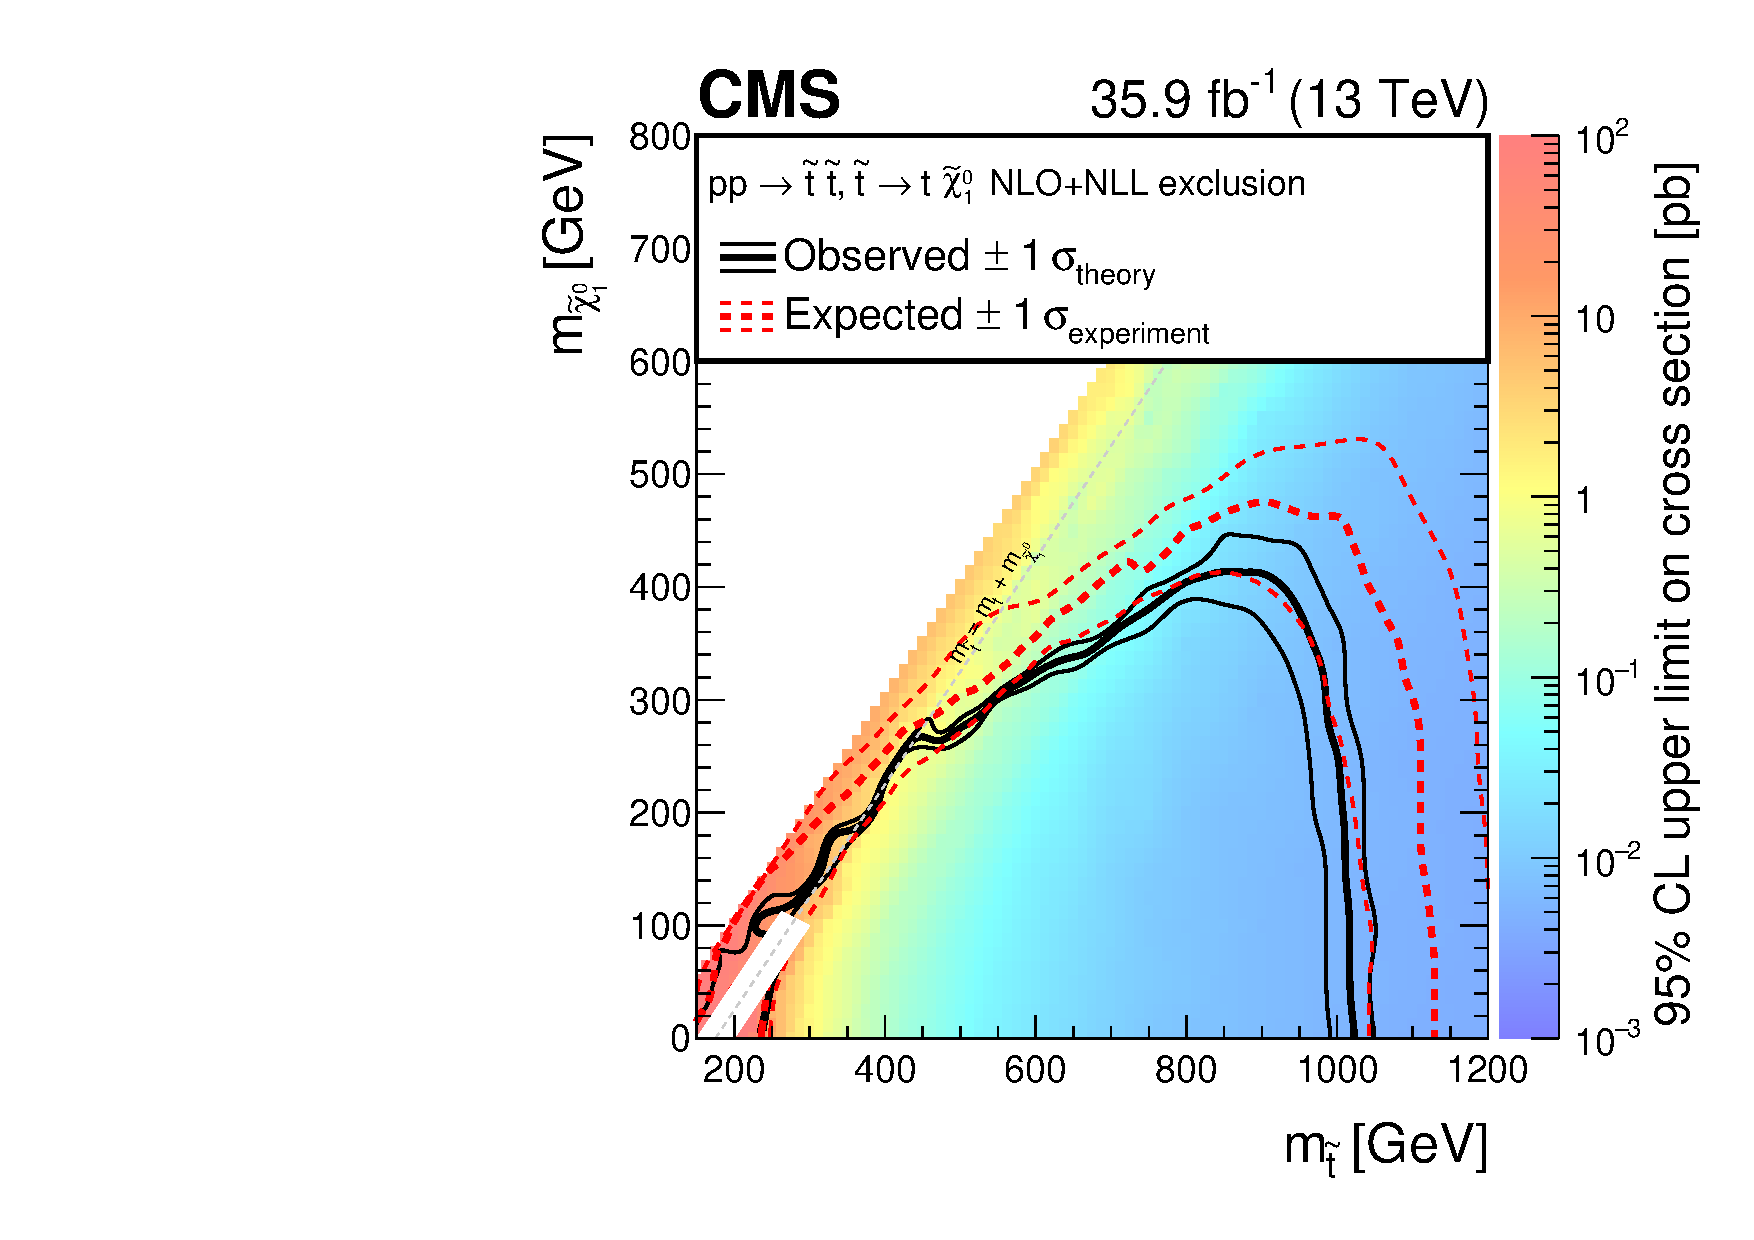
\includegraphics[width=0.50\textwidth]{sections/mc4/Results/figures/Covered_T2tt_OnlyXSEC.pdf}\\
  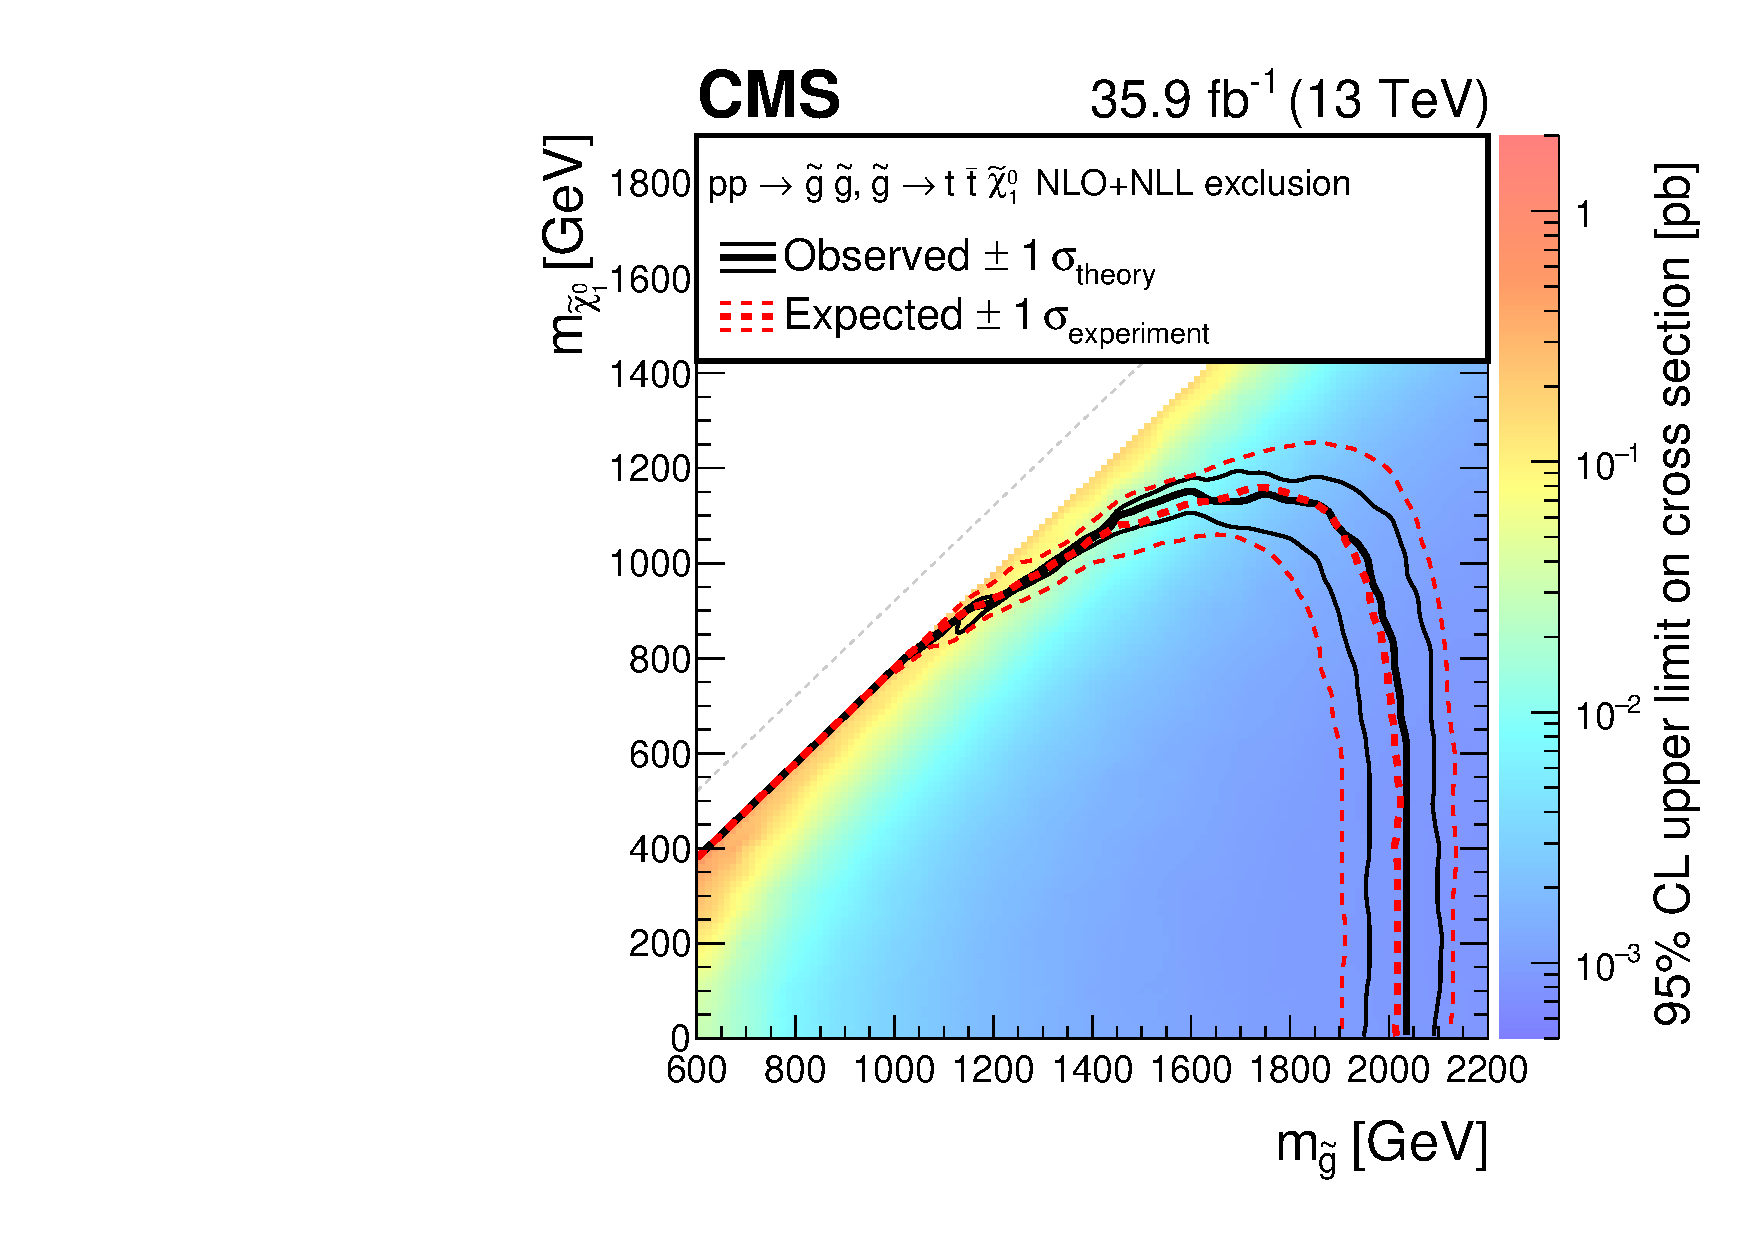
\includegraphics[width=0.40\textwidth]{sections/mc4/Results/figures/T1tttt_OnlyXSEC.pdf}
  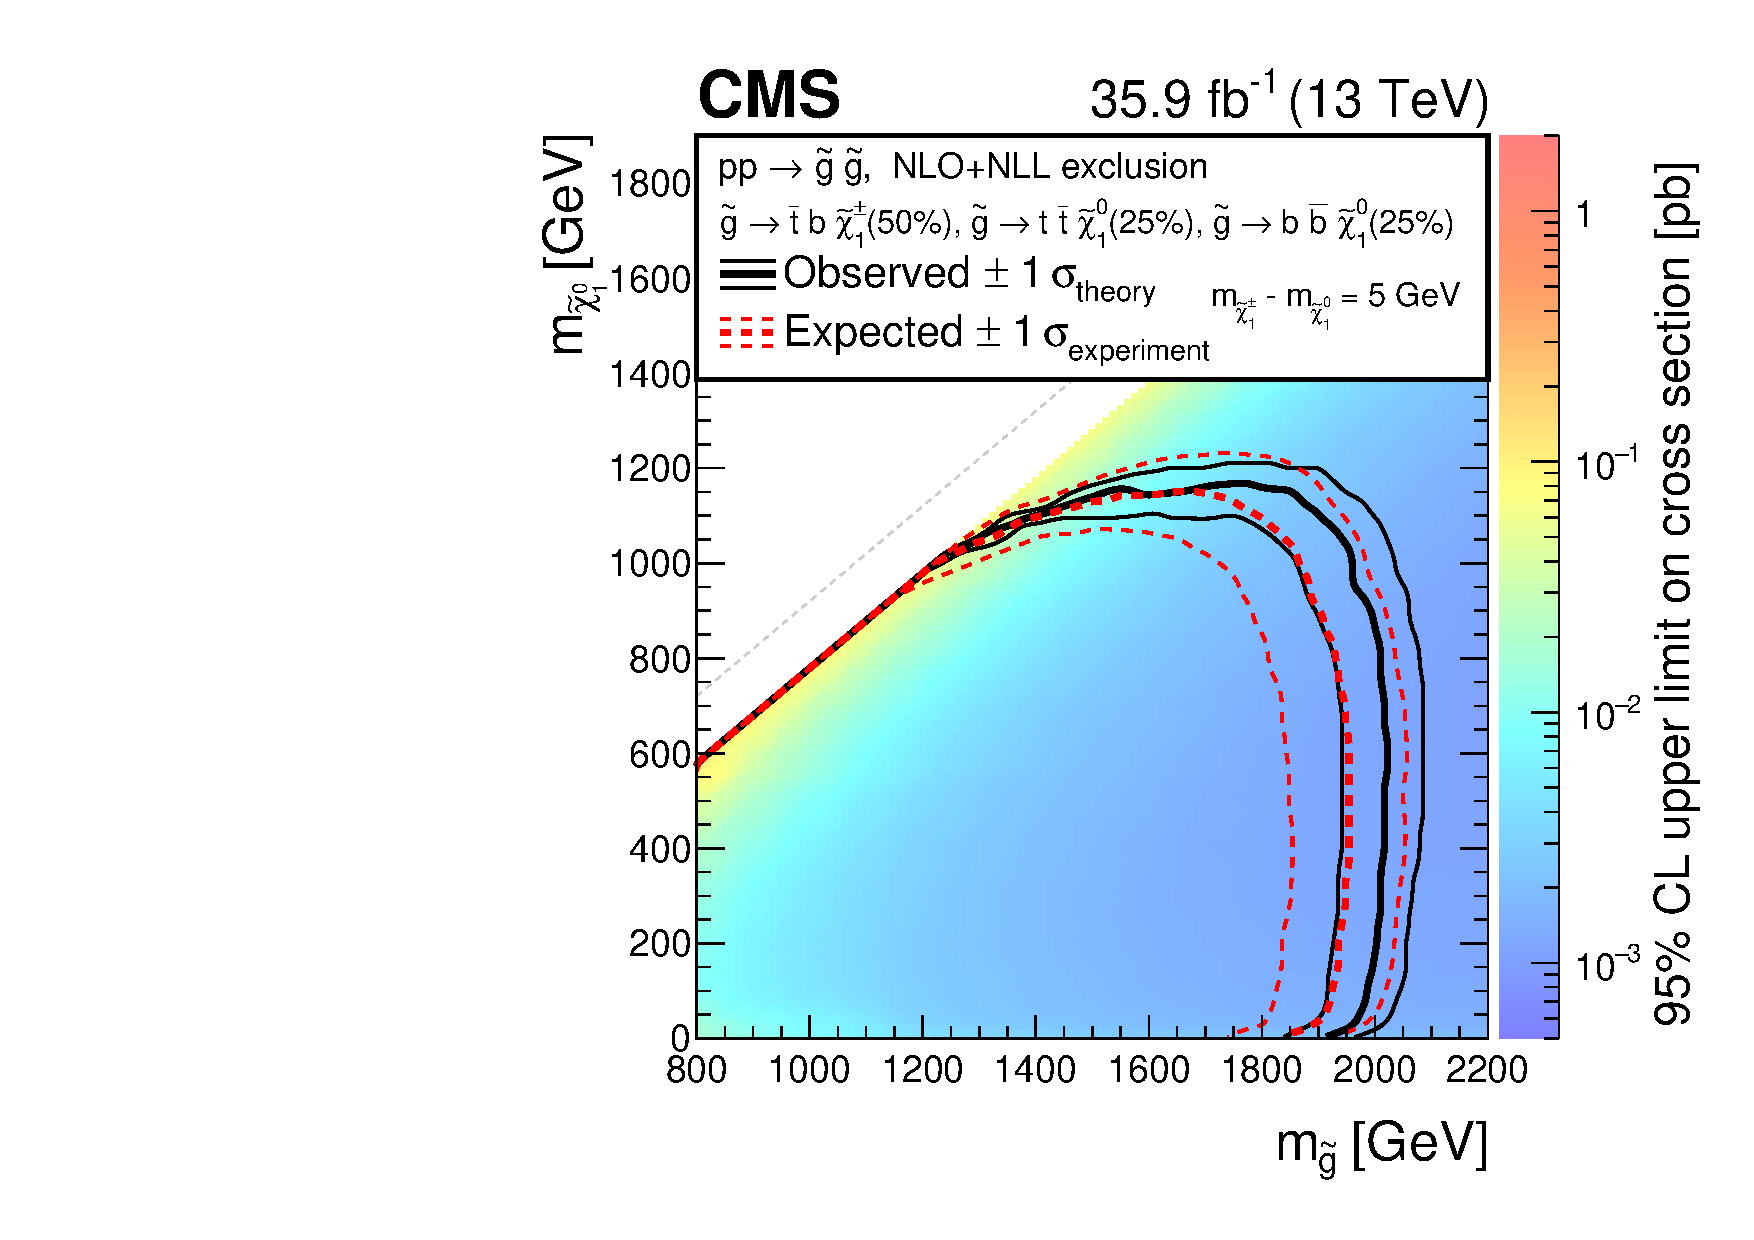
\includegraphics[width=0.40\textwidth]{sections/mc4/Results/figures/T1ttbb_OnlyXSEC.pdf}\\
  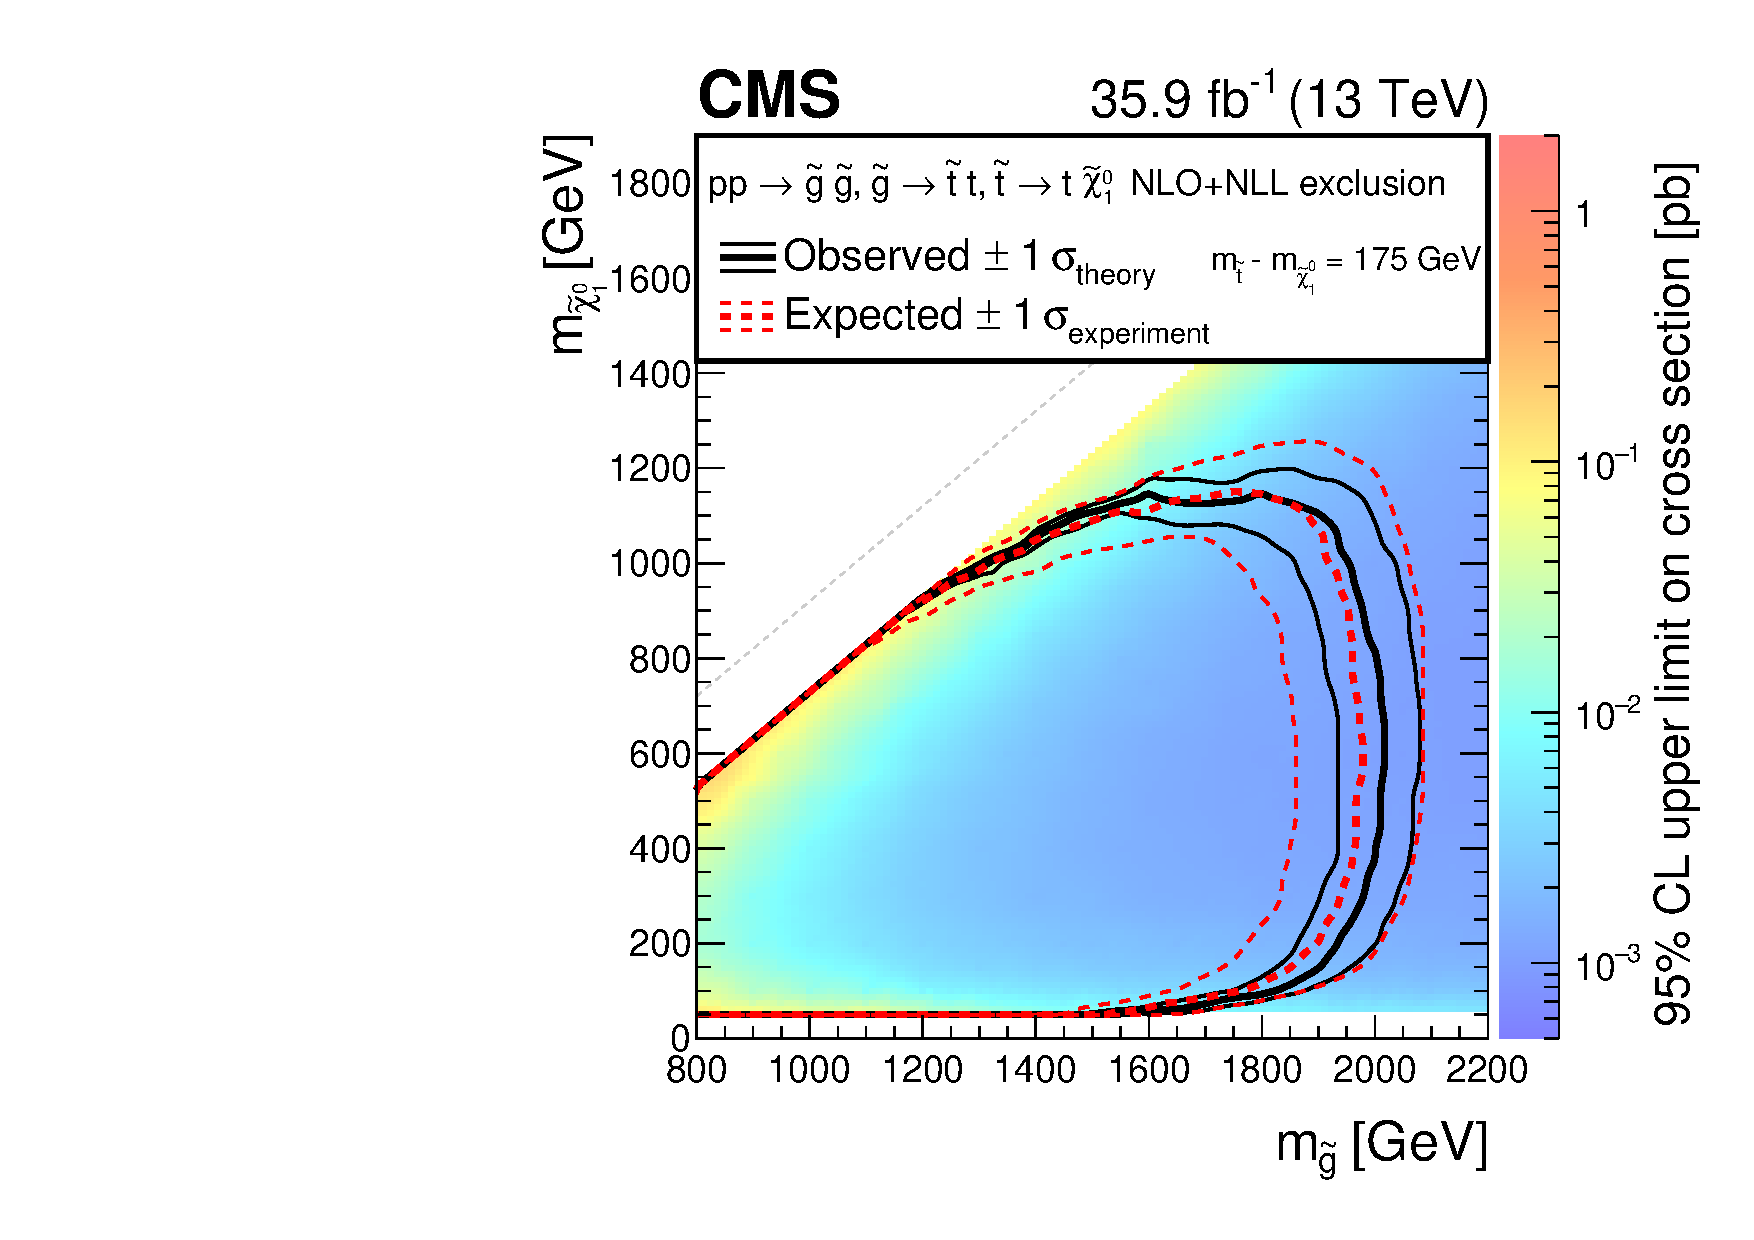
\includegraphics[width=0.40\textwidth]{sections/mc4/Results/figures/T5ttttdM175_OnlyXSEC.pdf}
  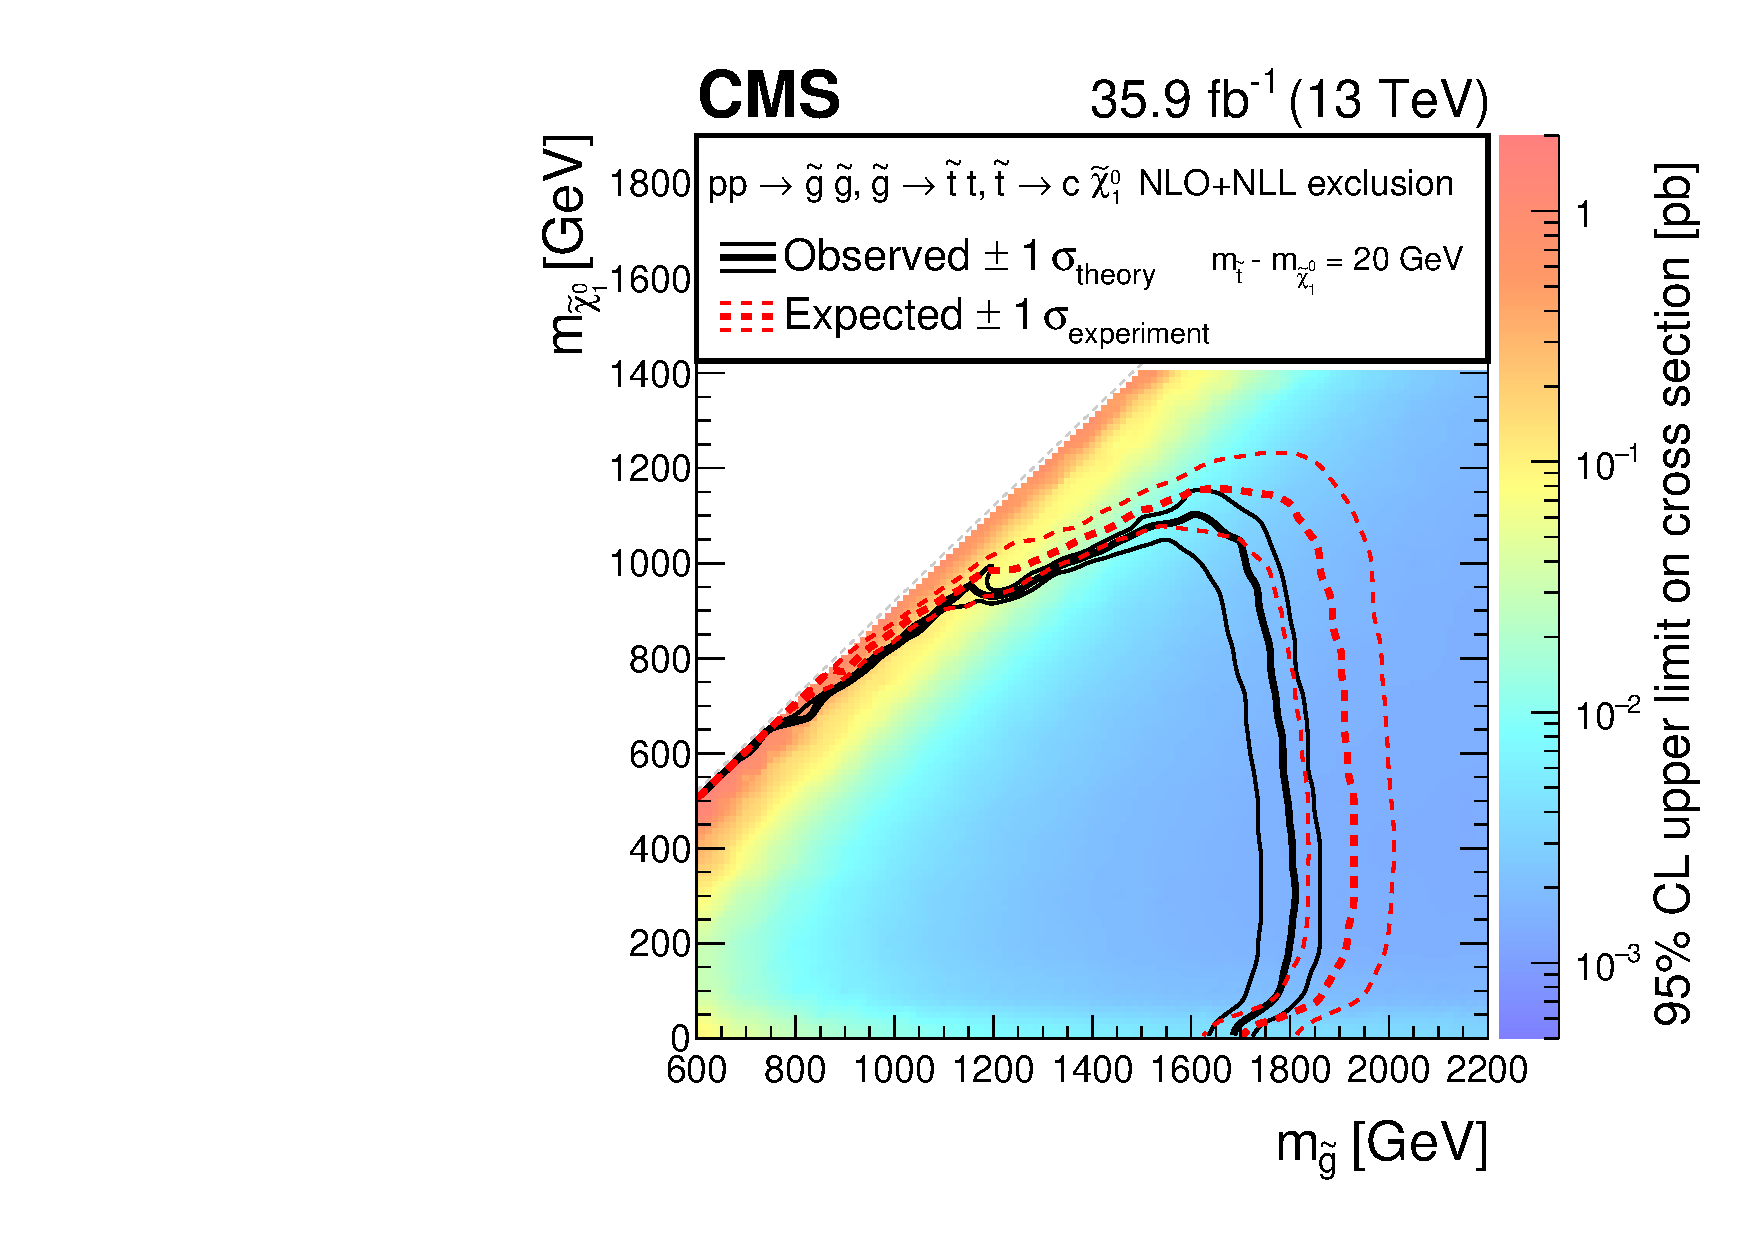
\includegraphics[width=0.40\textwidth]{sections/mc4/Results/figures/T5ttcc_OnlyXSEC.pdf}\\
  \caption{Exclusion limit at 95\% CL for the signal models in this search: top squark pair production with the top squark decaying into a top quark and neutralino (top), and top squarks from cascade decays of gluinos (middle and bottom). The top is T2tt, the middle left model as T1tttt, middle right model as T1ttbb the bottom left one as T5tttt and the bottom right one as T5ttcc.}
  \label{fig:signal_diagrams}
 \end{centering}
\end{figure}

The exclusion limits on the model parameters are summarized in Table~\ref{tab:c4limitsummary}:

\begin{table}[htbp]
\fontsize{10 pt}{1.2 em}
\selectfont
\begin{centering}
\caption{\label{tab:c4limitsummary} Expected Exclusion summary table}
\hspace*{-4ex}
\begin{tabular}{|c|c|c|}
\hline
SMS Model & \specialcell{LSP mass \\ expected exclusion} & \specialcell{SUSY Mother mass \\ expected exclusion} \\
\hline
T2tt & 430 GeV & 1020 GeV \\
\hline
T1tttt & 1100 GeV & 2040 GeV \\
\hline
T1ttbb & 1150 GeV & 1900 GeV \\
\hline
T5tttt & 1100 GeV & 1950 GeV \\
\hline
T5ttcc & 1120 GeV & 1940 GeV \\
\hline
\end{tabular}
\par\end{centering}
\end{table}
